\chapter{Approximating the burning sequence}\label{chapter:approximation}

\section{Approximation for general graphs}

Bessy et. al. \cite{Bessy2017} have given a 3-approximation algorithm for burning of an arbitrary graph. \Cref{algorithm:generate-burning-sequence} (in combination with \Cref{procedure:choose-last-fire-source}) is able to compute a burning sequence for a graph $G$ in $O(n^3)$ time, where $n=|G.V|$.

\begin{procedure}\label{procedure:choose-last-fire-source}
Given the input $(G,k,S)$ where $G$ is the input graph, $k$ is a positive integer, and $S$ is a burning sequence of size $k-1$, perform the following steps.
\end{procedure}

\textbf{\textit{Stage 1.}} $x_k = \max\{\min\{\frac{d(u,x_j)}{k-j+1}: j\in [1:i-1]\} : u\in G.V \}$.

\textbf{\textit{Stage 2.}} $S=S \cup_{s/} (x_k)$. Return $S$.\\

\begin{algorithm}\label{algorithm:generate-burning-sequence}
Given the input graph $G$, perform the following steps.
\end{algorithm}

\textbf{\textit{Stage 1.}} $x_1 =$ some arbitrary vertex. $S=(x_1)$.

\textbf{\textit{Stage 2.}} $\forall\ k\geq 2$, perform the following steps.

\textbf{\textit{Stage 2.1.}} Invoke \Cref{procedure:choose-last-fire-source} by passing the input $(G,k,S)$ and store the return value in $S$. If $S$ satisfies \cref{equation:burn-verify}, then stop and return $S$.\\

We show in \Cref{lemma:burn-seq-geq3} and \Cref{theorem:proof-3-approx} \cite{Bessy2017} that the burning sequence generated by \Cref{algorithm:generate-burning-sequence} is a burning sequence within 3-approximation. It means that (since graph burning is a minimization problem) if \Cref{algorithm:generate-burning-sequence} generates a burning sequence of length $k$, then an optimal burning sequence (generated by \Cref{algorithm:burn-general-optimal}) of the subject graph $G$ shall contain at least $\frac{k}{3}$ fire sources.

\begin{lemma}\label{lemma:burn-seq-geq3}
Let $S = (x_1, x_2, x_3, . . ., x_k)$ be a burning sequence returned by \cref{procedure:choose-last-fire-source} for an input graph $G$. If $S$ is not able to burn $G$ completely (that is, if $S$ does not satisfy \Cref{equation:burn-verify}), then $b(G)\geq \big\lceil \frac{k}{3}\big\rceil+1$.
\end{lemma}

\begin{proof}
If $S$ does not satisfy \Cref{equation:burn-verify}, then $\exists$ a vertex $u$ such that

$$\min \Big\{ \frac{dist(u,x_j)}{k-j+1} : j\in [k]\Big\} \geq 1$$.

$\forall\ i,j \in [k], i<j$, we have that $dist(i,j) \geq k-j+1 > k-j$. Now $\because j>i$, we have that $k-j > \big\lceil\frac{k-j}{2}\big\rceil + \big\lceil\frac{k-i}{2}\big\rceil$, we obtain that the $k$ sets\\
$N_{\lceil \frac{k-1}{2}\rceil}[x_1], N_{\lceil \frac{k-2}{2}\rceil}[x_2], N_{\lceil \frac{k-3}{2}\rceil}[x_3], . . ., N_0[x_{k}]$\\
are pairwise disjoint.

Now let (for contradiction) that a burning sequence of length $S^\prime = (y_1, y_2, y_3, . . ., y_{k^\prime})$ of length $k^\prime$ is able to burn $G$, where $k^\prime\leq \big\lfloor\frac{k}{3}\big\rfloor$.

$\because$ the ``half'' neighbourhood of the first $\big\lfloor\frac{k}{3}\big\rfloor+1$ fire sources is more than the neighbourhood of the first fire source (the fire source with the maximum neighbourhood reachability) that is,\\
$$\bigg\lceil\frac{k-\big\lceil\frac{k}{3}\big\rceil-1}{2}\bigg\rceil \geq \big\lfloor\frac{k}{3}\big\rfloor-1 \geq k^\prime-1,$$\\
then each of the (first) $\big\lfloor\frac{k}{3}\big\rfloor+1$ sets\\
$N_{\lceil \frac{k-1}{2}\rceil}[x_1], N_{\lceil \frac{k-2}{2}\rceil}[x_2], N_{\lceil \frac{k-3}{2}\rceil}[x_3], . . ., N_{\bigg\lceil\frac{k-\big\lceil\frac{k}{3}\big\rceil-1}{2}\bigg\rceil}\bigg[x_{\big\lceil\frac{k}{3}\big\rceil+1}\bigg]$

\noindent contain at least one element from $S^\prime$. $\because$ all these sets are pairwise disjoint, we obtain the contradiction to our assumption because $S^\prime$ will not be able to burn $G$. So $S^\prime$ must contain at least one more fire source.
\end{proof}

\begin{theorem}\label{theorem:proof-3-approx}
Let $S = (x_1, x_2, x_3, . . ., x_k)$ be a burning sequence returned by \Cref{algorithm:generate-burning-sequence}, then $b(G) \geq \frac{k}{3}$.
\end{theorem}

\begin{proof}
If \Cref{algorithm:generate-burning-sequence} returns a burning sequence of length $k$, then procedure 24 must not have been able to burn $G$ with $k-1$ fire sources.\\
$\implies$ (from \Cref{lemma:burn-seq-geq3}) $b(G) \geq \big\lceil \frac{k-1}{3}\big\rceil+1 \geq \frac{k}{3}$.
\end{proof}

\section{How close can we approximate?}\label{section:no-better-than-3-approx}

Let that for a given arbitrary graph $G,\ S = (x_1, x_2, x_3, . . ., x_k)$ be a burning sequence returned by an arbitrary approximation algorithm $A$ in polynomial time. If for a pair of fire sources $x_i, x_j$ their neighbourhoods are disjoint then the following expression satisfies.
$$\big | G.N_{k-i} [x_i] \cap G.N_{k-j}[x_j] \big | = 0.$$\\
If for a pair of fire sources $x_i, x_j$ it is observed that the $f^{th}$ fraction ($0 \leq f \leq 1$) of their neighbourhoods are disjoint then the following expression satisfies.
$$\big | G.N_{\lceil f \times (k-i) \rceil} [x_i] \cap G.N_{\lceil f \times (k-j)\rceil}[x_j] \big | = 0.$$\\
So, ``half'' neighbourhoods (where $f=\frac{1}{2}$) of any two distinct fire sources $x_i$ and $x_j$ are disjoint iff
$$\Big |\ G.N_{\big\lceil\frac{k-i}{2}\big\rceil}[x_i] \cap G.N_{\big\lceil\frac{k-j}{2}\big\rceil}[x_j]\ \Big | = 0.$$

By \Cref{lemma:b(SP)} (in \Cref{section:burn-general-graphs-optimally}), we have that $b(SP(s, r)) = r+1$ if $s \geq r$; if $s \geq r+2$, then the first fire source $y_1$ of the optimal burning sequence $S^{\prime} = (y_1, y_2, y_3, . . ., y_{k^{\prime}})$ must be placed on its head node $c$.\\

If some algorithm $A$ claims that uptil it is not able to burn $G$, the $f$-fraction neighbourhood of all pairs of fire sources are disjoint, then, the following expression satisfies for all values of $k \in \mathbb{N}$ uptil which $A$ is not able to burn $G$.
$$\big | G.N_{\lceil f \times (k-i) \rceil} [x_i] \cap G.N_{\lceil f \times (k-j)\rceil}[x_j] \big | = 0,$$ $\forall\ 1 \leq i, j \leq k, i \neq j$.\\

\begin{lemma}\label{lemma:half-neighbourhood-limit-SP}
Let $S = (x_1, x_2, . . ., x_k)$ be a burning sequence returned by an approximation algorithm for $SP(d,k^{\prime}-1)$, $d \geq k^{\prime}+1$, the maximum burning neighbourhood fraction that it claim to be pairwise disjoint is the half neighbourhood for all pairs of fire sources uptil $SP(d,k^{\prime}-1)$ is not burnt, that is,  $\forall\ 1 \leq i, j \leq k-1, i \neq j$,\\
$$\Big |\ G.N_{\big\lceil\frac{k-i}{2}\big\rceil}[x_i] \cap G.N_{\big\lceil\frac{k-j}{2}\big\rceil}[x_j]\ \Big | = 0.$$
\end{lemma}

\begin{proof}
Let $S^{\prime} = (y_1, y_2, . . ., y_{k^{\prime}})$ be an optimal burning sequence for $SP(\infty, k^{\prime}-1)$. In a spider graph $SP(d, k^{\prime}-1)$, we know by lemma 12 in \cite{Bessy2017} that the first fire source $y_1$ will always be kept on the head vertex $c$, also observe that\\
$\because k^{\prime} > \big (\big\lceil\frac{k^{\prime}-1}{2}\big\rceil + 1 \big ) + \big (\big\lceil\frac{k^{\prime}-2}{2}\big\rceil + 1 \big )$,\\
$\implies \Big |\ N_{\big\lceil\frac{k^{\prime}-1}{2}\big\rceil}[y_1] \cap N_{\big\lceil\frac{k^{\prime}-2}{2}\big\rceil}[y_2]\ \Big | \geq 1$\\
if $y_2$ is placed on any vertex in $G.V \setminus \{c\}$.

Let that we are only supplied by a burning sequence of $S^{\prime\prime} = (y_1^{\prime}, y_2^{\prime}, . . ., y_{k^{\prime}-1}^{\prime})$ length $k^{\prime}-1$ to burn $SP(d, k^{\prime}-1)$. Let us assume that $c$ is still the fixed place for the first fire source $y_1^{\prime}$. Then,\\
$\because k^{\prime} \geq \big (\big\lceil\frac{k^{\prime}-2}{2}\big\rceil + 1 \big ) + \big (\big\lceil\frac{k^{\prime}-3}{2}\big\rceil + 1 \big )$,\\
$\implies \Big |\ N_{\big\lceil\frac{k^{\prime}-2}{2}\big\rceil}[y_1^{\prime}] \cap N_{\big\lceil\frac{k^{\prime}-3}{2}\big\rceil}[y_2^{\prime}]\ \Big | \geq 0$\\
if $y_2^{\prime}$ is placed on any vertex in $G.V \setminus \{c\}$.

Also observe that if the neighbourhood fraction is increased, then,\\
$\because k^{\prime} > \big (\big\lceil\frac{k^{\prime}-1}{2}\big\rceil + \epsilon + 1 \big ) + \big (\big\lceil\frac{k^{\prime}-2}{2}\big\rceil + \epsilon + 1\big )$,\\
$\implies \Big |\ N_{\big\lceil\frac{k^{\prime}-2}{2} \big\rceil + \epsilon}[y_1^{\prime}] \cap N_{\big\lceil\frac{k^{\prime}-3}{2} \big\rceil + \epsilon}[y_2^{\prime}]\ \Big | \geq 1$\\
if $y_2^{\prime}$ is placed on any vertex in $G.V \setminus \{c\}$ given that $\epsilon$ has a positive value.

This implies that if $S = (x_1, x_2, . . ., x_k)$ is a burning sequence of length $k \geq k^{\prime}$ returned by an arbitrary $z$-approximation algorithm on $SP(d,k^{\prime})$, $z \geq 1+\varepsilon, \varepsilon > 0\ (\implies k^{\prime} \leq k \leq (1 + \varepsilon) \times k^{\prime})$, then the algorithm can make sure that for any pair of distinct fire sources computed by it, $x_i, x_j, i \neq j$, a maximum of half neighbourhood is disjoint when it will be/was restricted to produce a sequence of length $k-1$, that is, for $1\leq i, j \leq k-1, i \neq j$\\
$$\Big |\ N_{\big\lceil\frac{k-1-i}{2} \big\rceil}[x_1] \cap N_{\big\lceil\frac{k-1-j}{2} \big\rceil}[x_2]\ \Big | = 0.$$

This implies the lemma.
\end{proof}

\begin{lemma}\label{lemma:3-approx-example}
    If an approximation algorithm is able to guarantee an $l$-fraction neighbourhood disjointness on all distinct pair of fire sources, $0 < l \leq 1/2$, until it burns a given graph $G$, it can only claim $z \geq 3$ approximation factor for burning general graphs.
\end{lemma}

\begin{proof}
\begin{figure}
	\begin{minipage}{1\textwidth}
		\centering
		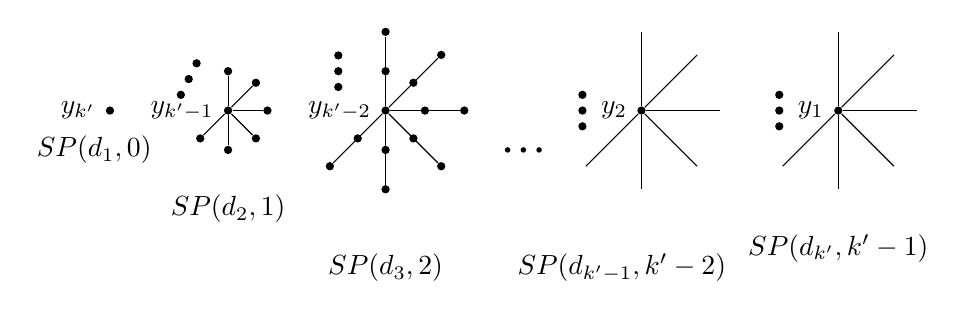
\begin{tikzpicture}
		    \node [circle, fill=black, inner sep=0pt, minimum size=3pt, label=left:{$y_{k^{\prime}}$}] at (-.5,0) {};
		    
		    
		    \node [circle, fill=black, inner sep=0pt, minimum size=3pt, label=left:{$y_{k^{\prime}-1}$}] (AA) at (1,0) {};
		    \node [circle, fill=black, inner sep=0pt, minimum size=3pt] (AB) at (1,0.5) {};
		    \node [circle, fill=black, inner sep=0pt, minimum size=3pt] (AC) at (1.3535,0.3535) {};
		    \node [circle, fill=black, inner sep=0pt, minimum size=3pt] (AD) at (1.5,0) {};
		    \node [circle, fill=black, inner sep=0pt, minimum size=3pt] (AE) at (1.3535,-0.3535) {};
		    \node [circle, fill=black, inner sep=0pt, minimum size=3pt] (AF) at (1,-.5) {};
		    \node [circle, fill=black, inner sep=0pt, minimum size=3pt] (AG) at (1-.3535,-0.3535) {};
		    
		    \node [circle, fill=black, inner sep=0pt, minimum size=3pt] at (1-.6,0.2) {};
		    \node [circle, fill=black, inner sep=0pt, minimum size=3pt] at (1-.5,0.4) {};
		    \node [circle, fill=black, inner sep=0pt, minimum size=3pt] at (1-.4,0.6) {};
		    
			\draw (AA) -- (AB);
			\draw (AA) -- (AC);
			\draw (AA) -- (AD);
			\draw (AA) -- (AE);
			\draw (AA) -- (AF);
			\draw (AA) -- (AG);
			
			
		    \node [circle, fill=black, inner sep=0pt, minimum size=3pt, label=left:{$y_{k^{\prime}-2}$}] (BA) at (3,0) {};
		    \node [circle, fill=black, inner sep=0pt, minimum size=3pt] (BB) at (3,0.5) {};
		    \node [circle, fill=black, inner sep=0pt, minimum size=3pt] (BC) at (3,1) {};
		    \node [circle, fill=black, inner sep=0pt, minimum size=3pt] (BD) at (3.3535,0.3535) {};
		    \node [circle, fill=black, inner sep=0pt, minimum size=3pt] (BE) at (3.707,0.707) {};
		    \node [circle, fill=black, inner sep=0pt, minimum size=3pt] (BF) at (3.5,0) {};
		    \node [circle, fill=black, inner sep=0pt, minimum size=3pt] (BG) at (3+1,0) {};
		    \node [circle, fill=black, inner sep=0pt, minimum size=3pt] (BH) at (3.3535,-0.3535) {};
		    \node [circle, fill=black, inner sep=0pt, minimum size=3pt] (BI) at (3.707,-0.707) {};
		    \node [circle, fill=black, inner sep=0pt, minimum size=3pt] (BJ) at (3,-0.5) {};
		    \node [circle, fill=black, inner sep=0pt, minimum size=3pt] (BK) at (3,-1) {};
		    \node [circle, fill=black, inner sep=0pt, minimum size=3pt] (BL) at (3-0.3535,-0.3535) {};
		    \node [circle, fill=black, inner sep=0pt, minimum size=3pt] (BM) at (3-0.707,-0.707) {};
		    
		    \node [circle, fill=black, inner sep=0pt, minimum size=3pt] at (3.5-1.1,.5) {};
		    \node [circle, fill=black, inner sep=0pt, minimum size=3pt] at (3.5-1.1,.3) {};
		    \node [circle, fill=black, inner sep=0pt, minimum size=3pt] at (3.5-1.1,.7) {};
		    
			\draw (BA) -- (BC);
			\draw (BA) -- (BE);
			\draw (BA) -- (BG);
			\draw (BA) -- (BI);
			\draw (BA) -- (BK);
			\draw (BA) -- (BM);
			
			\node [circle, fill=black, inner sep=0pt, minimum size=2pt] at (5-.25,-.5) {};
		    \node [circle, fill=black, inner sep=0pt, minimum size=2pt] at (5.2-.25,-.5) {};
		    \node [circle, fill=black, inner sep=0pt, minimum size=2pt] at (5-0.2-.25,-.5) {};
			
			
		    \node [circle, fill=black, inner sep=0pt, minimum size=3pt, label=left:{$y_2$}] (CA) at (7-.75,0) {};
		    
		    \node [circle, fill=black, inner sep=0pt, minimum size=3pt] at (7-1.5,0) {};
		    \node [circle, fill=black, inner sep=0pt, minimum size=3pt] at (7-1.5,-0.2) {};
		    \node [circle, fill=black, inner sep=0pt, minimum size=3pt] at (7-1.5,0.2) {};
		    
			\draw (CA) -- (7-.75,1);
			\draw (CA) -- (7.707-.75,0.707);
			\draw (CA) -- (7+1-.75,0);
			\draw (CA) -- (7.707-.75,-0.707);
			\draw (CA) -- (7-.75,-1);
			\draw (CA) -- (7-0.707-.75,-0.707);
			
			\node [circle, fill=black, inner sep=0pt, minimum size=3pt, label=left:{$y_1$}] (DA) at (8.75,0) {};
		    
		    \node [circle, fill=black, inner sep=0pt, minimum size=3pt] at (9-1,0) {};
		    \node [circle, fill=black, inner sep=0pt, minimum size=3pt] at (9-1,-0.2) {};
		    \node [circle, fill=black, inner sep=0pt, minimum size=3pt] at (9-1,0.2) {};
		    
			\draw (DA) -- (8.75,1);
			\draw (DA) -- (8.75+.707,0.707);
			\draw (DA) -- (8.75+1,0);
			\draw (DA) -- (8.75+.707,-0.707);
			\draw (DA) -- (8.75,-1);
			\draw (DA) -- (8.75-0.707,-0.707);
			
			\node at (-.7,-.5) {$SP(d_1 ,0)$};
			\node at (1,-1.25) {$SP(d_2 ,1)$};
			\node at (3,-2) {$SP(d_3 ,2)$};
			\node at (6,-2) {$SP(d_{k^{\prime}-1} ,k^{\prime}-2)$};
			\node at (8.75,-1.75) {$SP(d_{k^{\prime}},k^{\prime}-1)$};
		\end{tikzpicture}
	\end{minipage}
	
	\caption{Burning of a graph with $k^{\prime}$ components $comp_i$. Each $comp_i$ having one central head vertex, has $d_i \geq i+1$ arms of equal length $i-i$. Burning number of this graph is $k^{\prime}$.}
\end{figure}

\begin{figure}
	\begin{minipage}{1\textwidth}
		\centering
		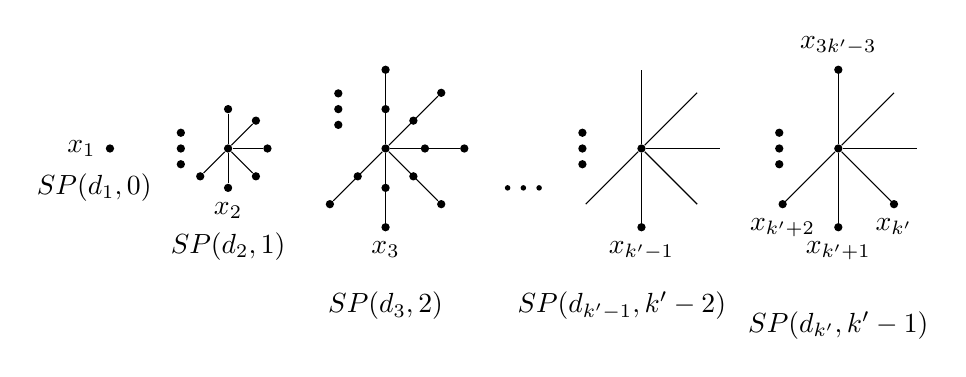
\begin{tikzpicture}
		    \node [circle, fill=black, inner sep=0pt, minimum size=3pt, label=left:{$x_1$}] at (-.5,0) {};
		    
		    
		    \node [circle, fill=black, inner sep=0pt, minimum size=3pt] (AA) at (1,0) {};
		    \node [circle, fill=black, inner sep=0pt, minimum size=3pt] (AB) at (1,0.5) {};
		    \node [circle, fill=black, inner sep=0pt, minimum size=3pt] (AC) at (1.3535,0.3535) {};
		    \node [circle, fill=black, inner sep=0pt, minimum size=3pt] (AD) at (1.5,0) {};
		    \node [circle, fill=black, inner sep=0pt, minimum size=3pt] (AE) at (1.3535,-0.3535) {};
		    \node [circle, fill=black, inner sep=0pt, minimum size=3pt, label=below:{$x_2$}] (AF) at (1,-.5) {};
		    \node [circle, fill=black, inner sep=0pt, minimum size=3pt] (AG) at (1-.3535,-0.3535) {};
		    
		    \node [circle, fill=black, inner sep=0pt, minimum size=3pt] at (1-.6,0) {};
		    \node [circle, fill=black, inner sep=0pt, minimum size=3pt] at (1-.6,-0.2) {};
		    \node [circle, fill=black, inner sep=0pt, minimum size=3pt] at (1-.6,0.2) {};
		    
			\draw (AA) -- (AB);
			\draw (AA) -- (AC);
			\draw (AA) -- (AD);
			\draw (AA) -- (AE);
			\draw (AA) -- (AF);
			\draw (AA) -- (AG);
			
			
		    \node [circle, fill=black, inner sep=0pt, minimum size=3pt] (BA) at (3,0) {};
		    \node [circle, fill=black, inner sep=0pt, minimum size=3pt] (BB) at (3,0.5) {};
		    \node [circle, fill=black, inner sep=0pt, minimum size=3pt] (BC) at (3,1) {};
		    \node [circle, fill=black, inner sep=0pt, minimum size=3pt] (BD) at (3.3535,0.3535) {};
		    \node [circle, fill=black, inner sep=0pt, minimum size=3pt] (BE) at (3.707,0.707) {};
		    \node [circle, fill=black, inner sep=0pt, minimum size=3pt] (BF) at (3.5,0) {};
		    \node [circle, fill=black, inner sep=0pt, minimum size=3pt] (BG) at (3+1,0) {};
		    \node [circle, fill=black, inner sep=0pt, minimum size=3pt] (BH) at (3.3535,-0.3535) {};
		    \node [circle, fill=black, inner sep=0pt, minimum size=3pt] (BI) at (3.707,-0.707) {};
		    \node [circle, fill=black, inner sep=0pt, minimum size=3pt] (BJ) at (3,-0.5) {};
		    \node [circle, fill=black, inner sep=0pt, minimum size=3pt, label=below:{$x_3$}] (BK) at (3,-1) {};
		    \node [circle, fill=black, inner sep=0pt, minimum size=3pt] (BL) at (3-0.3535,-0.3535) {};
		    \node [circle, fill=black, inner sep=0pt, minimum size=3pt] (BM) at (3-0.707,-0.707) {};
		    
		    \node [circle, fill=black, inner sep=0pt, minimum size=3pt] at (3.5-1.1,.5) {};
		    \node [circle, fill=black, inner sep=0pt, minimum size=3pt] at (3.5-1.1,.3) {};
		    \node [circle, fill=black, inner sep=0pt, minimum size=3pt] at (3.5-1.1,.7) {};
		    
			\draw (BA) -- (BC);
			\draw (BA) -- (BE);
			\draw (BA) -- (BG);
			\draw (BA) -- (BI);
			\draw (BA) -- (BK);
			\draw (BA) -- (BM);
			
			\node [circle, fill=black, inner sep=0pt, minimum size=2pt] at (5-.25,-.5) {};
		    \node [circle, fill=black, inner sep=0pt, minimum size=2pt] at (5.2-.25,-.5) {};
		    \node [circle, fill=black, inner sep=0pt, minimum size=2pt] at (5-0.2-.25,-.5) {};
			
			
		    \node [circle, fill=black, inner sep=0pt, minimum size=3pt] (CA) at (7-.75,0) {};
		    
		    \node [circle, fill=black, inner sep=0pt, minimum size=3pt] at (7-1.5,0) {};
		    \node [circle, fill=black, inner sep=0pt, minimum size=3pt] at (7-1.5,-0.2) {};
		    \node [circle, fill=black, inner sep=0pt, minimum size=3pt] at (7-1.5,0.2) {};
		    
		    \node [circle, fill=black, inner sep=0pt, minimum size=3pt, label=below:{$x_{k^{\prime}-1}$}] at (7-.75,-1) {};
		    
			\draw (CA) -- (7-.75,1);
			\draw (CA) -- (7.707-.75,0.707);
			\draw (CA) -- (7+1-.75,0);
			\draw (CA) -- (7.707-.75,-0.707);
			\draw (CA) -- (7-.75,-1);
			\draw (CA) -- (7-0.707-.75,-0.707);
			
			\node [circle, fill=black, inner sep=0pt, minimum size=3pt] (DA) at (8.75,0) {};
		    
		    \node [circle, fill=black, inner sep=0pt, minimum size=3pt] at (9-1,0) {};
		    \node [circle, fill=black, inner sep=0pt, minimum size=3pt] at (9-1,-0.2) {};
		    \node [circle, fill=black, inner sep=0pt, minimum size=3pt] at (9-1,0.2) {};
		    
		    \node [circle, fill=black, inner sep=0pt, minimum size=3pt, label=below:{$x_{k^{\prime}}$}] (BK) at (8.75+.707,-.707) {};
		    \node [circle, fill=black, inner sep=0pt, minimum size=3pt, label=below:{$x_{k^{\prime}+1}$}] (BK) at (8.75,-1) {};
		    \node [circle, fill=black, inner sep=0pt, minimum size=3pt, label=below:{$x_{k^{\prime}+2}$}] (BK) at (8.75-0.707,-0.707) {};
		    \node [circle, fill=black, inner sep=0pt, minimum size=3pt, label=above:{$x_{3 k^{\prime}-3}$}] (BK) at (8.75,1) {};
		    
			\draw (DA) -- (8.75,1);
			\draw (DA) -- (8.75+.707,0.707);
			\draw (DA) -- (8.75+1,0);
			\draw (DA) -- (8.75+.707,-0.707);
			\draw (DA) -- (8.75,-1);
			\draw (DA) -- (8.75-0.707,-0.707);
			
			\node at (-.7,-.5) {$SP(d_1 ,0)$};
			\node at (1,-1.25) {$SP(d_2 ,1)$};
			\node at (3,-2) {$SP(d_3 ,2)$};
			\node at (6,-2) {$SP(d_{k^{\prime}-1} ,k^{\prime}-2)$};
			\node at (8.75,-2.25) {$SP(d_{k^{\prime}} ,k^{\prime}-1)$};
		\end{tikzpicture}
	\end{minipage}
	
	\caption{Burning of a graph with $k^{\prime}$ components $comp_i$. Each $comp_i$ having one central head vertex, has $d_i \geq i+1$ arms of equal length $i-i$. A burning sequence of length $3 k^{\prime}-3$ is shown to not to be able to burn $SP(X)$ completely.}
\end{figure}

As shown in figure 2, $SP(X)$ is a disjoint union of spider graphs $SP(d_1, 0)$, $SP(d_2, 1)$, $SP(d_3, 2)$, $. . .$, $SP(d_{k^{\prime}-1}, k^{\prime}-2)$, and $SP(d_{k^{\prime}}, k^{\prime}-1)$; $d_i \geq i+1$.

The construction of a burning sequence $S$ (not optimal) for $SP(X)$ for a fixed $k^{\prime}$ is as follows. $\forall\ i, 1 \leq i \leq k^{\prime}-2$, a fire source $x_i$ is placed on one of the leaf nodes of $SP(d_i, i-1)$. $\forall\ k^{\prime} \leq i \leq 3k^{\prime}-3$ a fire source $x_i$ is placed on a distinct leaf node of $SP(d_{k^{\prime}}, k^{\prime}-1)$ where no other fire source is already placed. Figure 1 demonstrates the construction of this burning sequence $S$ for $SP(X)$, which may be returned by an arbitrary approximation algorithm $A$.

For $1 \leq k \leq 3 k^{\prime}-3$, if a burning sequence $S=(x_1, x_2, x_3, . . ., x_k)$ is used to burn the graph and the fire sources $\{x_i\}$ are placed according to the preceding procedure, then we can observe that $S$ is not able to burn $SP(X)$, and for all the fire sources, their $0 < l \leq 1/2$ factor neighbourhood is disjoint with each other. Also, it is trivially observable that if the value of $l$ decreases, then the number of required fire source will increase accordingly.
\end{proof}

Let $G$ be an arbitrary graph, and $S = (x_1, x_2, . . ., x_k)$ be a burning sequence of length $k$ returned by an arbitrary $z$-approximation algorithm $A$, $z \geq 1+\varepsilon, \varepsilon > 0$. Let $b(G) = k^{\prime}$.

From the proofs of \Cref{lemma:half-neighbourhood-limit-SP} and \Cref{lemma:3-approx-example}, we have that if $A$ will be/was restricted to produce a burning sequence of length $l \leq k-1$ for an arbitrary $G$ if $k \geq k^{\prime}$, it can be claimed that $\forall\ x_i, x_j, 1 \leq i, j \leq k-1, i \neq j,$
$$\Big |\ N_{\big\lceil\frac{l-i}{2} \big\rceil + \epsilon}[x_1] \cap N_{\big\lceil\frac{l-j}{2} \big\rceil + \epsilon}[x_2]\ \Big | = 0$$\\
only if $\epsilon \leq 0$. It means that for an approximation algorithm for general graph burning, the upper bound of $\epsilon$ is 0.

This is the maximum that $A$ can claim for a general graph. Let that $A$ is able to guarantee this. It means that if $G$ is not burnt completely and $\epsilon \leq 0$, then $A$ guarantees that\\
$N_{\lceil\frac{k-1}{2}\rceil}[x_1], N_{\lceil\frac{k-2}{2}\rceil}[x_2], N_{\lceil\frac{k-3}{2}\rceil}[x_3], . . ., N_0[x_k]$ are pairwise disjoint, and\\
$\because \Bigg\lceil \frac{k-\big\lceil\frac{k}{3}\big\rceil-1}{2} \Bigg\rceil \geq \big\lfloor \frac{k}{3} \big\rfloor-1$,\\
$\implies b(G) \leq \big\lfloor\frac{k}{3}\big\rfloor+1$ (by \Cref{lemma:burn-seq-geq3}).\\
$\implies z \geq 3 \implies \varepsilon = 2$ (by \Cref{theorem:proof-3-approx}).

These properties allow us to suggest that graph burning may be hard to approximate better than the $3$-approximation ratio, which we formally state as \Cref{conjecture:no-better-than-3-approx} as follows.

\begin{conjecture}\label{conjecture:no-better-than-3-approx}
    A maximum of 3-approximation is possible in polynomial time to compute burning number of general graphs.\qed
\end{conjecture}

If it is a necessary attribute for an approximation algorithm for burning general graphs to claim a neighbourhood factor disjointness between each pair of fire sources in the burning sequence $S = (x_1, x_2, . . ., x_k)$ returned by it, then a maximum of 3-approximation is possible in polynomial time to compute burning number of general graphs.

\section{Approximating the burning of connected interval graphs}

We discussed in \Cref{subsection:IG-path-similar} that if $P$ is the diameter of an interval graph $G$, then all the other vertices in $G$, that is, the vertices in $G\setminus P$, are connected to at least one vertex in $P$ by a single edge.
We discussed in \Cref{section:burn-path} that we can burn a path optimally in polynomial time using \Cref{algorithm:burn-path-finite}. Following from this we discussed in \Cref{subsection:similar-burn-path-IG} that the burning number of an interval graph $G$ $b(P)\leq b(G)\leq b(P)+1$. We showed in \Cref{section:burn-interval-graphs} that determining whether $b(G)=b(P)$ is NP-Complete. We describe \Cref{algorithm:approximate-burn-IG} as follows, which is able to burn an interval graph $G$ within $b(G)+1$. We have used the \textsc{Algebraic-Floyd-Warshall} \cite{Kepner2011} to compute $P$, the diameter of $G$, which is a shortest path of maximum length in $G$.

\begin{algorithm}\label{algorithm:approximate-burn-IG}
    Given an interval graph $G$, perform the following steps.
\end{algorithm}

\textbf{\textit{Stage 1.}} $F=$ a set of shortest paths between all pairs of vertices from the \textsc{Algebraic-Floyd-Warshall} algorithm. $P=$ a path of maximum length in $F$.

\textbf{\textit{Stage 2.}} Invoke \Cref{algorithm:burn-path-finite} by passing $(G, P)$ as input, store the return value in $S=(x_1,x_2,\dots,x_k)$.

\textbf{\textit{Stage 3.}} If $S$ is not able to burn $G$ completely, that is, if $S$ does not satisfy \Cref{equation:burn-verify}, then $v=$ an arbitrary vertex in $G.V\setminus (G.N_{k-1}[x_1]\cup G.N_{k-2}[x_2]\cup\dots\cup G.N_0[x_k])$. $S=S\cup_{s/}v$.

\textbf{\textit{Stage 4.}} Return $S$.\\

Time complexity of \Cref{algorithm:approximate-burn-IG} is $O(n)$, where $n$ is the number of vertices in $G$. $S$ is the burning sequence returned by \Cref{algorithm:approximate-burn-IG}.

In \Cref{section:inapproximability-NPH}, we discussed in \Cref{theorem:approximability-general} that no approximation algorithm $A$ can guarantee an approximation ratio $R_A$ of less than $k+(1/k)$ if $k$ is the cost of the optimal solution of a problem $P$ on some input $x$. If the burning number of a connected interval graph $G$ be $k=b(G)$, \Cref{algorithm:approximate-burn-IG} is able to approximate burning of interval graphs within $k+1$. Thus we get that the approximation ratio for burning interval graphs is $R_A=k+(1/k)$.

% \bibliography{ref.bib}
% \bibliographystyle{plain}